\chapter{Postsynaptic Model}
\label{chap:Postsynaptic-models}

Study of central synapses is hampered by inaccessibility, rapid kinetics, and
difficulty of measuring and/or controlling the time course of neurotransmitter.

The time course of neurotransmitter in the synaptic cleft has been known to be
very brief (Sect.\ref{sec:neurotransmitter-time-course}), and the kinetics of
the postsynaptic receptors are responsible for the slower time-course of the
postsynaptic currents.  Upon the neurotransmitter release
(Chap.\ref{chap:Presynaptic-models}), it will triggers the opening of the
receptor on the postsynaptic side. For Glutamate, it activates two different
kinds of receptors: AMPAR (Chap.\ref{chap:AMPAR-models}) and NMDAR
(Chap.\ref{chap:NMDAR_models}).


The components on postsynaptic side is discussed in
Sect.\ref{sec:postsynaptic-side-structure} and Sect.\ref{sec:both-side-synapse}.

\begin{enumerate}
  \item model the general classes of receptors and their prototypical properties
  \item model the subtypes of receptors:
  
there exists a considerable range of physiological subtypes, and depending upon
the subtypes, it can gives rise to different properties of receptors
\begin{itemize}
  \item NMDAR depends on NR2 subunit (Sect.\ref{sec:NMDAR}) for $\Mg$
  sensitivity and kinetics of the channel.
  
  \item AMPAR depends on the presence of GluR-B for $\Ca$ permeability (Jonas
  et al., 1994); and both (GluR-B and GluR-D) for channel desensitization
  (Mosbacher et al., 1994).

Example: Interneurons express faster, more $\Ca$-permeable AMPAR than principal
neurons (Geiger et al., 1995).

  \item 
\end{itemize}
\end{enumerate}

\section{Synaptic efficacy}
\label{sec:synaptic-efficacy}


Synaptic efficacy is a basic concept in neuroscience that refers to the capacity
of a presynaptic input to influence postsynaptic output.
The synaptic efficacy is a measure of the strength of a given synaptic
connection.

It is typically not able to measured directly at the synapse level, but from the
somata. So, the increase/decrease in the recorded signal in the soma can be the
result of one or many factors

\begin{itemize}

  \item \textcolor{red}{pre-synaptic factor}:
  \begin{enumerate}
  \item the increase/decrease in the number of release sites $n$, 
  
  \item the increase/decrease in the probability of neurotransmitter release
  $P_r$, making AMPAR  opening more/less effectively: 
  \end{enumerate}
  
  \item \textcolor{red}{post-synaptic factor}
  (Sect.\ref{sec:synaptic-efficacy-post-synaptic-factors})

  \begin{enumerate}
  \item the increase/decrease of the postsynaptic signal (EPSP for excitatory
  or IPSP for inhibitory)
  
  \end{enumerate} 
\end{itemize}

Several experimental studies tried to control the condition to record the signal
from only one synapse, and suggesting the synaptic efficacy recorded comes from
post-synaptic side {\it per se}. This raises the question: what changes from the
post-synaptic side that increase the efficacy (leading to LTP) or decrease the
efficacy (leading to LTD)?

\subsection{Pre-synaptic factors}
\label{sec:synaptic-efficacy-pre-synaptic-factors}

\subsection{Post-synaptic factors}
\label{sec:synaptic-efficacy-post-synaptic-factors}

Is is assumed that there is no change in pre-synaptic release (each release we
get the same amount of neurotransmitter). The synaptic efficacy can be
represented as
\begin{itemize}
  \item  a fraction of opening channel $r$, which can be AMPAR or NMDAR
  
  \item NMDAR impose a weight $w$ on AMPAR.
\end{itemize}


\subsection{- Hebbian: spike trains}
\label{sec:synaptic-efficacy-pre-synaptic-factors-Hebbian-square-wave-instant-response} 

The synaptic efficacy can be represented as a fraction of opening channel $r$.
Here, it assumes (1) square wave form of neurotransmitter, (2) instantaneous
response of postsynaptic efficacy.

The gating of post-synaptic receptor (e.g. AMPAR)
\begin{equation}
\ce{C <=>[a_1(\Vm,[L])][a_2(\Vm)] O}
\end{equation}
with $[L]$ is concentration of neurotransmitter
(Sect.\ref{sec:neurotransmitter-time-course}). 

Assume the kinetic rates are constant, or subject to a step transition
(e.g. ligand-gated current in subject to a pulse of transmitter or
voltage-dependent current in respond to a voltage clamp).

Given $r$ is the fraction of opening channels
\begin{equation}
\frac{dr}{dt} = a_1 (\Vm,[L]) \times (1-r) - a_2 r
\end{equation}

Steady-state value:
\begin{itemize}
  \item if we assume 
\begin{equation}
\begin{array}{cc}
\Vm = V_0; [L]=L_0 & \text{ if } t < t_0 \\
\Vm = V_1; [L]=L_1 & \text{ if } t < t_1 \\
\end{array}
\end{equation}

Then
\begin{equation}
r(t-t_o) = r_\infty + K_1 \exp(-\frac{t-t_o}{\tau_1})
\end{equation}
with $K_1 = r_o - r_\infty$.
\begin{equation}
\begin{split}
r_\infty = \frac{a_1(V_1,[L]_1)}{a_1(V_1,[L]_1)+a_2 (V_1)} \\
\tau_1 = \frac{1}{a_1(V_1,[L]_1)+a_2 (V_1)}
\end{split}
\end{equation}

  \item If we assume a square wave pulse of [L] (Sect.\ref{sec:neurotransmitter-time-course})
and
\begin{equation}
\ce{C <=>[\alpha . L][\beta ] O}
\end{equation}

\def\pre{{\text{pre}}}
\def\post{{\text{post}}}

Then
\begin{equation}
\begin{split}
r_\infty = \frac{[L]_\max}{[L]_\max+K_s} \\
\tau_1 = \frac{1}{[L]_\max+K_s}
\end{split}
\end{equation}
with $K_s = \beta/\alpha$. At the end of the pulse, then 
\begin{equation}
r_\post = r_\infty + (r_\pre - r_\infty) e^{-\Delta t/\tau}
\end{equation}
with $r_\pre$ is the fraction of channel open just before the pulse; and 
$r_\post$ is the fraction of channel open after the end of the square wave
pulse.

\end{itemize}
%Here: [L]=0 at most of the time; and [L] = $L_o$ at $t=t_o$ (time at which
%neurotransmitter are released).

If the neurotransmitter pulse is short, e.g. $\Delta t \approx 1$ms, 
$r$ cannot reach steady state value. To prove that, we can define
\begin{verbatim}
r^-  as the value of 'r' just before the spike, at time t^-
r^+  as the value of 'r' just after the spike, at time t^+
\end{verbatim}
then
\begin{equation}
S_+ = S_- + (1 - S_- ) (1- e^{-\gamma})
\end{equation}
and for the first spike it reaches the value
$S_+ \approx 0.63$ with $\gamma = 1$ which is not saturate (i.e. not 1).
After the spike it decays exponentially. In a spike train, we can model using

\begin{equation}
\frac{dr}{dt} = \alpha \sum_i \delta(t-t_i) (1-r) - \frac{r}{\tau_i}
\end{equation}
with $t_i$ is the time at which a pulse $i-$th occurs with the corresponding
time constant $\tau_i$.

As $r$ is bound between 0 and 1, the mean synaptic efficacy $r$ deviates from
linear and starting to saturate when the presynaptic firing rate $r$ is much
larger than $1/\tau_s$. We can consider the synaptic efficacy specifically for
different types of receptors
\begin{itemize}
  \item $\tau_s = 2	$ (ms) for AMPAR
  \item $\tau-s = 100$ (ms) for NMDAR
\end{itemize}

\begin{figure}[hbt]
  \centerline{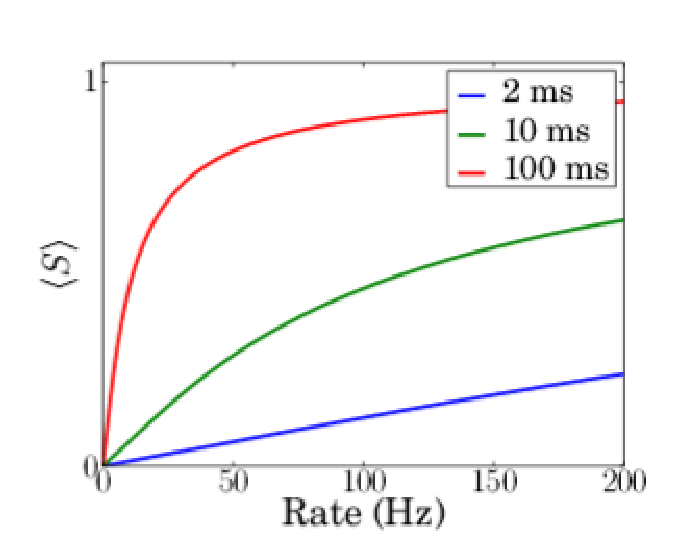
\includegraphics[height=3cm,
    angle=0]{./images/synaptic-efficacy-presynaptic-firing-rates.eps}}
\caption{Saturation of synaptic efficacy as a function of firing rates}
\label{fig:synaptic-efficacy-presynaptic-firing-rates}
\end{figure}




\subsection{- Hebbian: spike trains (more realistic)}

In the previous section
(Sect.\ref{sec:synaptic-efficacy-pre-synaptic-factors-Hebbian-square-wave-instant-response}),
we modeled with the assumption that synapses are opened instantaneously when a
presynaptic action potential occur.

A model like in Fig.\ref{fig:post-synaptic-response} captures a more realistic
response. A smooth rise time can be modeled using second-order kinetics, by
adding an additional variable $x$ follow first-order kinetics.
Second-order kinetics are used to produce a slow onset and decay with different
time constants.

\begin{enumerate}
  \item Method 1

\begin{equation}
\begin{split}
\frac{dr}{dt} = \alpha \times x \times (1-r) - \beta \times r \\
\frac{dx}{dt} = \alpha_x \times \sum_i \delta (t-t_i-\tau_L) - \beta_x \times
x
\end{split}
\end{equation}  
with $\tau_L$ (ms) is the time delay in the update of $x$, $t_i$ is the time
for the synaptic input.

$\tau_x = 1/\beta_x$ is the time constant for $x$ decays.
$\tau_r = 1/\beta_r$ is the time constant for $r$ decays.

If saturation can be neglected, i.e. no upper bound for $r$, then
Fig.\ref{fig:post-synaptic-response} is estimated by the curve
\begin{equation}
r(t) = \text{peak} \times \left( e^{-t/\tau_x} - e^{-t/\tau_r}\right)
\end{equation}
and the time-to-peak is 
\begin{equation}
\text{time-2-peak} = \frac{\ln\left( \frac{\tau_r}{\tau_x}\right)}{1/\tau_x -
1/\tau_r}
\end{equation}
with $\tau_r > \tau_x$.
  \item Method 2:

\begin{equation}
\begin{split}
\frac{dr}{dt} = \alpha \times x \times (1-r) - \beta \times r \\
\frac{dx}{dt} = \alpha_x \times F(V_\pre) (1-x) - \beta_x \times x
\end{split}
\end{equation}
with $\alpha_i $ (unit: 1/msec).
\begin{equation}
F(V_\pre) = \frac{1}{1+ \exp(-V_\pre/2.0)}
\end{equation}

\end{enumerate}

\begin{figure}[hbt]
  \centerline{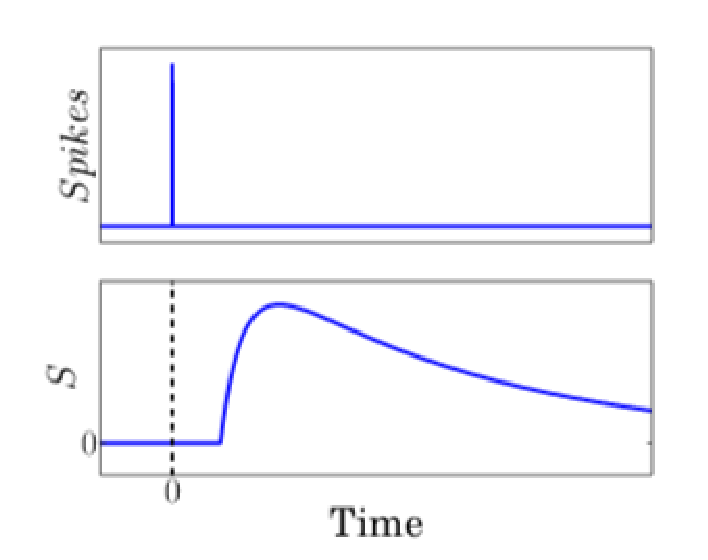
\includegraphics[height=3cm,
    angle=0]{./images/post-synaptic-response.eps}}
\caption{A more realistic response behavior of postsynaptic efficacy}
\label{fig:post-synaptic-response}
\end{figure}


\subsection{- STDP}

Phenomenological models formularize the synaptic efficacy as a dynamic variable
$\rho$
\begin{enumerate}
  
  \item  $[\Ca]_\post$ (via NMDAR) only:
  
  Graupner-Brunel (2002): first-order ODE with 4 terms, in which (1) two
  stable states via cubic function, (2) $\Ca$ elevation is the only factor
  controlling synaptic efficacy with $\Ca$-elevation caused by pre-synaptic
  signal contribute to LTP; while $\Ca$-elevation caused by post-synaptic signal
  (via bAP for example) contribute to LTD; (3) noise effects -
  Sect.\ref{sec:Graupner-Brunel-2012}.
  
  \item
\end{enumerate}

\subsection{Pre- and Post-synaptic factors}

Here, we need to dynamically model neurotransmitter concentration [NT]
as a function of pre-synaptic voltage $V_\pre$.

The gating of AMPAR and NMDAR is a directly function of [NT].

\subsection{Synaptic information
efficacy (SIE)}

London et al. proposed a new functional measure of the mutual information shared
by the pre- and postsynaptic spike trains.

They  model postsynaptic output as a continuous string of '1's and '0's,
depending on whether or not the post-synaptic cell fired a spike at any given
point. In such a condition, there is a large degree of  uncertainty about
whether the next symbol in the string will be a '0' or a '1'.


\section{Measure synaptic strength}

% \ref{sec:synaptic-strength-measure}
% {\bf How a synaptic strenght is measured?}

\subsection{in ANN}

{\bf In artificial neural network} (ANN)
(Sect.\ref{sec:ANN-articial-neuron-network}): Mathematically, $w_{k.ij}$
represent the synaptic weight between neuron $i$ in layer (k) to neuron $j$ in
layer (k+1), Sect.\ref{sec:synaptic_plasticity-ANN}. It means that the effect
from a neuron in the previous layer on the neuron on the next layer can be
changed. The different formulas for updating this synaptic strength in ANN is
discussed in Sect.\ref{sec:learning}.
% , a neuron is a point neuron, i.e. no explicit synapse, so a single neuron has
% one synaptic strength, and this value is updated based upon the current
% synaptic strengths of neurons connecting to the given neuron.

\subsection{in nerve cell}
\label{sec:synaptic-strength-measure}
\label{sec:synaptic-strength}

There are different types of synapses, but chemical synapse is the most
important in the brain (Sect.\ref{sec:synapse}).
Upon neurotransmitters released from presynaptic terminal, they bind to the
different receptors on the postsynaptic side, and trigger the opening of these
ion channels (in the case of inotropic channels) or trigger intracellular
signaling cascade (in the case of metabotropic channels).

For inotropic channels, the influx currents
(Sect.\ref{sec:postsynaptic-current}) via these channels cause a membrane
depolarization that has a chance to trigger the postsynaptic potential
(Sect.\ref{sec:postsynaptic_potential}).

\textcolor{red}{From the experimental point of view}: measuring the
postsynaptic current at a single synapse is very difficult
(Sect.\ref{sec:postsynaptic-current}).

{\bf In real neurons}, the synaptic strength is not measured at individual
synapse level, but at the soma, given that the total input at soma is not enough to
trigger the spike. It is recorded as EPSC (Sect.\ref{sec:EPSC}).

\subsection{ * measure individual synaptic strength (synaptic efficacy)}

Some experiments done on large synapses, e.g. calyx of Held in mammalian
auditory system (Sect.\ref{sec:synapse-calyx-of-Held}), where the synaptic
current is measured using voltage clamp protocol. Here, we can measure the
current at single synapse (in nA) and the peak representing the synaptic weight
or synaptic strength.

\begin{figure}[hbt]
 \centerline{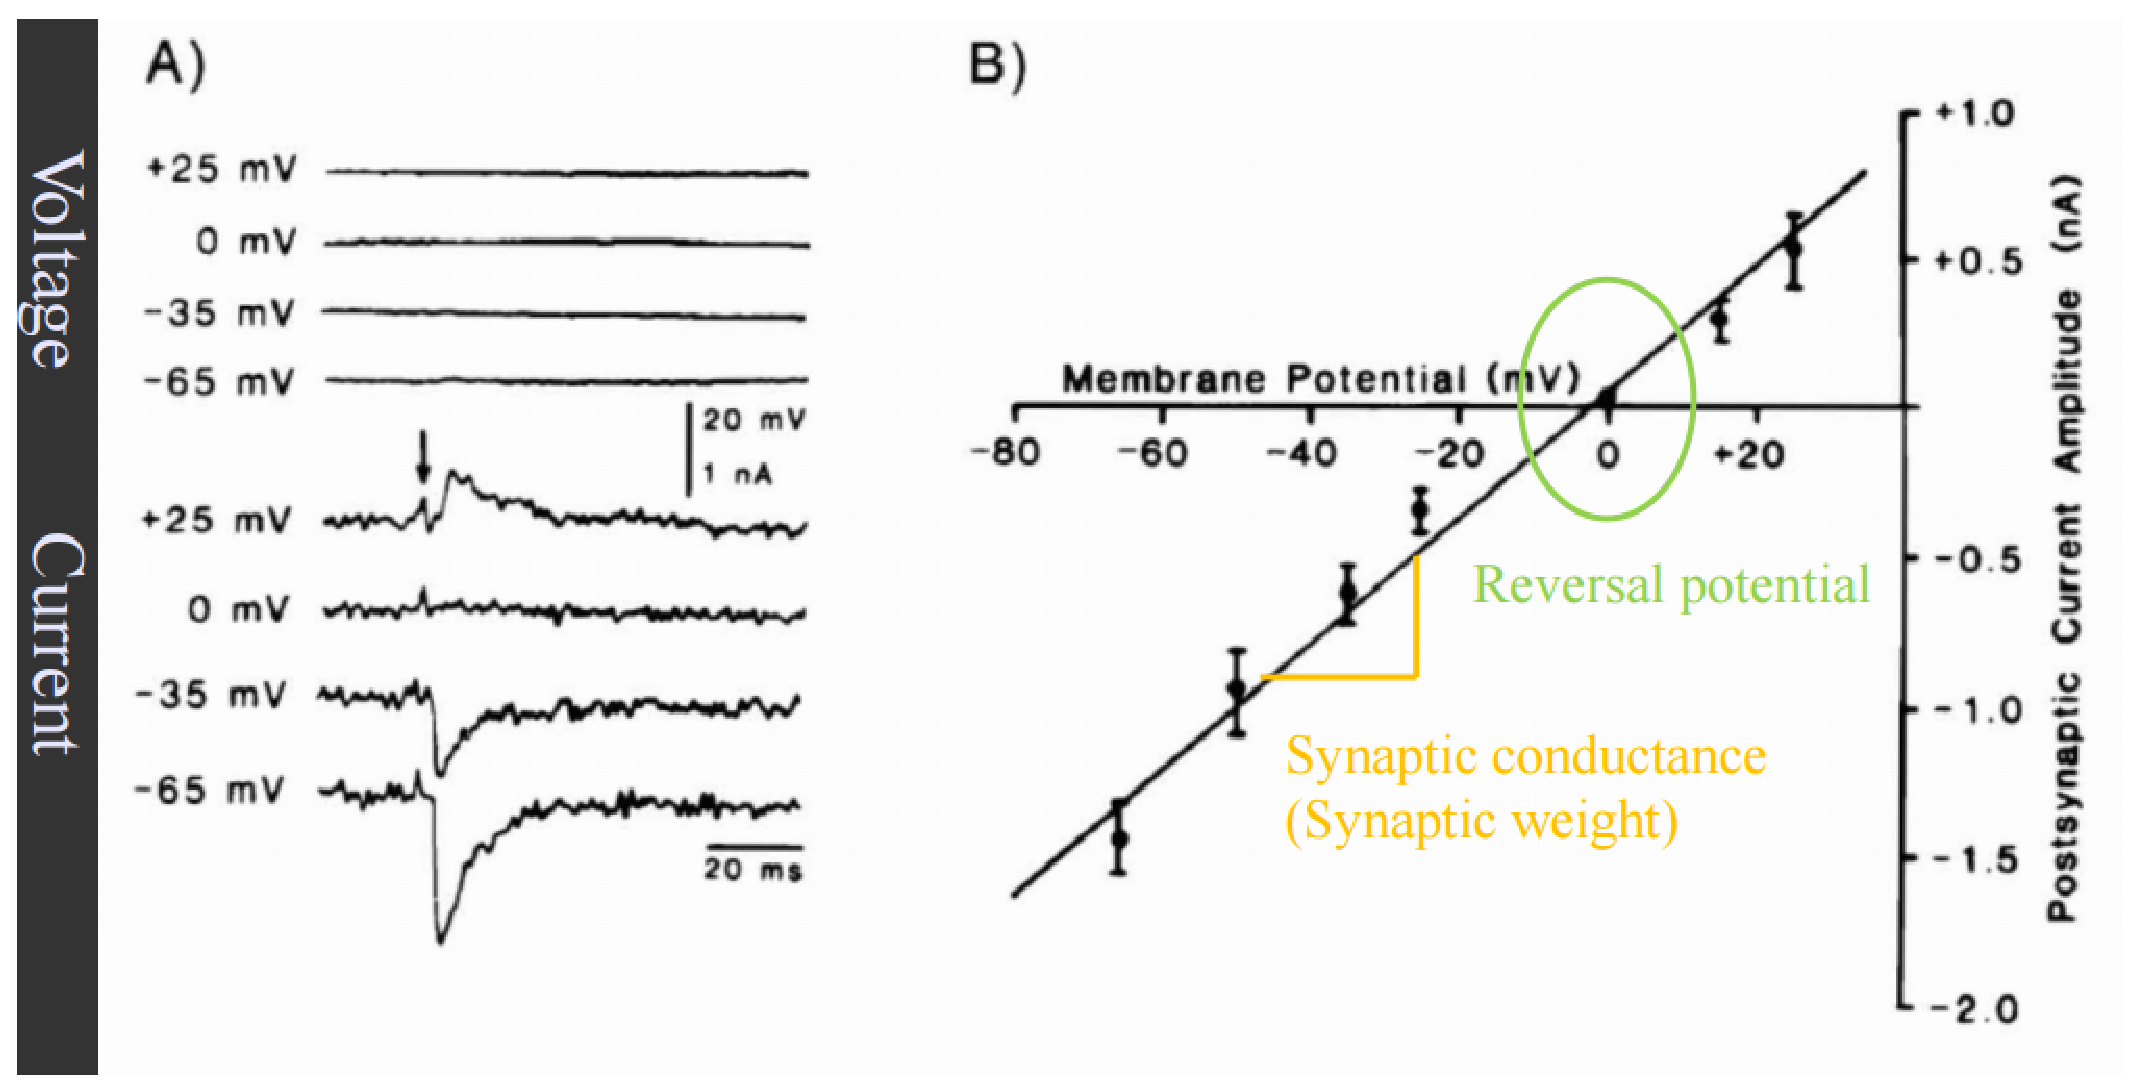
\includegraphics[height=5cm]{./images/synapse-voltage-current-curve.eps}}
 \caption{(A) the different postsynaptic membrane voltage clamp (in mV), and the
 recorded current (in nA) generated at postsynaptic side; (B) the I-V curve
 showing the peak current at different voltage clamp}
\label{fig:synapse-voltage-current-curve}
\end{figure}

\begin{figure}[htb]
    \centerline{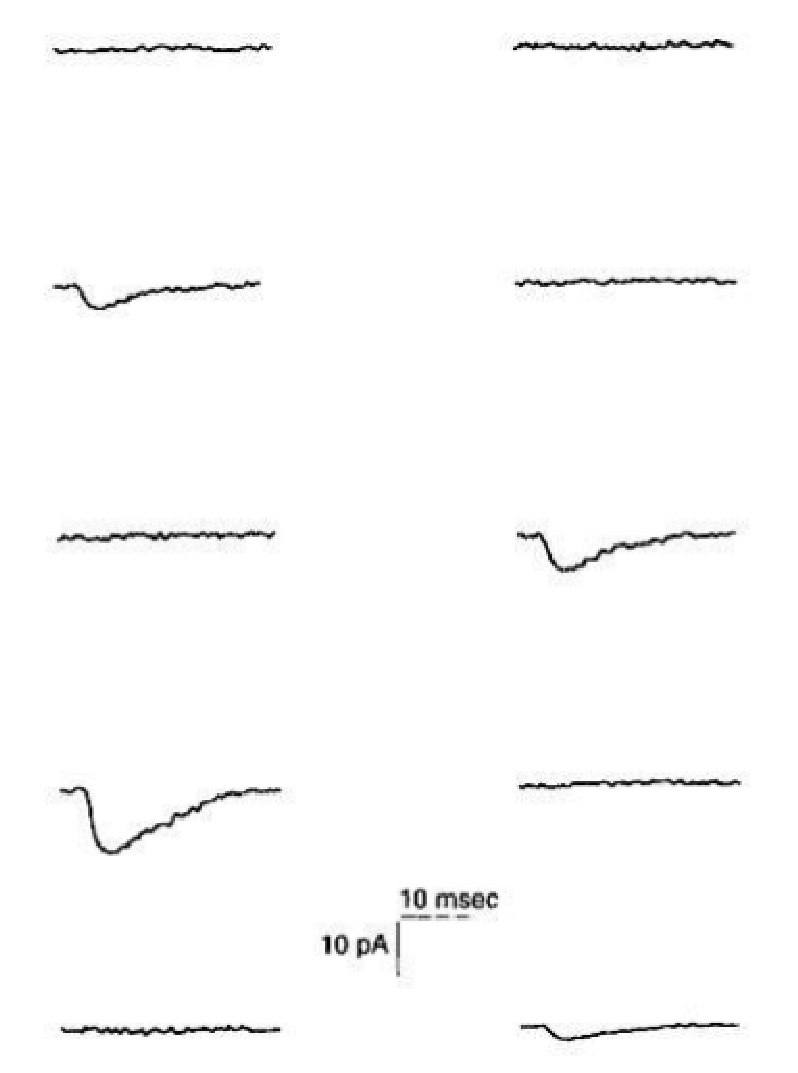
\includegraphics[height=5cm]{./images/PSC_trials.eps}}
    \caption{Postsynaptic current (PSC) is the result of
    stochastic opening of the proteins with an opening
    probability that can change depending on the membrane
    potential $V_m$}\label{fig:PSC_trials}
\end{figure}


Fig.\ref{fig:PSC_trials} shows the measured currents from 10 different trials
with
\begin{itemize}
  \item the opening of channels follows stochastic nature
  
  \item different size of EPSC: if channels openning
\end{itemize}
As a result, the {\bf average synaptic efficacy} is used to represent the
strength of a synapse in published experimental papers.

The change in the probability of triggering the postsynaptic potential is called
the synaptic plasticity (Sect.\ref{sec:synaptic_plasticity}). As the synaptic
strength refers to the efficacy that postsynaptic current can trigger
postsynaptic potential, it is also called {\bf synaptic efficacy}.
 
% The concept of synaptic strength in the brain is represented differently.
% Here, it is called the {\bf synaptic efficacy} and can be represented as

\textcolor{red}{From modelling and experimental point of view}, the synaptic
strength can be quantified as postsynaptic potential or postsynaptic current
(Sect.\ref{sec:synaptic-strength}).
\begin{itemize}
  \item the amplitude of individual postsynaptic potential (PSP) -
  Sect.\ref{sec:postsynaptic_potential}: EPSP or IPSP

In short-term potentiation, \textcolor{red}{the synaptic efficacy is measured in
the form of excitatory postsynaptic potential (EPSP) - Sect.\ref{sec:EPSP} in
the neuron, and postsynaptic end-plate potential (EPP) in the skeletal muscle
fiber in the case of  neuromuscular junction.}
  
  \item the amplitude of individual postsynaptic current (PSC) - 
  Sect.\ref{sec:postsynaptic-current}: EPSC or IPSC.
  
\end{itemize}


\textcolor{red}{From the modelling point of view}: depending on what approach we
use
\begin{enumerate}
  \item Deterministic approach: the meaning of synaptic strength is used as in
  experiment
  
  \item Stochastic approach: as we can simulate the stochastic activity of
  thousands of synapses for a single neuron at the same time, we can model
  accurately the variation in the recorded currents at different synapses.
\end{enumerate}

\subsection{pair-pulse ratio (PPR): Measuring the level of change in synaptic
efficacy}
\label{sec:pair-pulse-ratio}

In pair-pulse protocol, the pair-pulse ratio (PPR) is used to estimate the
change in synaptic efficacy (Sect.\ref{sec:synaptic-efficacy}) at different
interval of the pulses.

In paired-pulse protocol, the facilitation or depression of
EPSC can be quantified as a ratio of subsequence EPSC strength, i.e. $A_2/A_1$.

\textcolor{red}{One way to calculate EPSC}:
\begin{equation}
\begin{split}
A_i &= \EPSC = k \left( [\Ca]_\text{presynaptic} \right)^4 \\ 
    &=  k(\text{[Ca2+]rest + [Ca2+]influx + [Ca2+]residual})^4
\end{split}
\end{equation}
with $k$ is a constant. NOTE: At EPSC2, [Ca2+]influx = 0

So
\begin{equation}
\text{PPR} = \frac{\EPSC_2}{\EPSC_1} = \text{(1 + [$\Ca$]residual /
[$\Ca$]influx)}^4 - 1
\end{equation}
If [Ca2+]local/[Ca2+]residual $\sim 6.25$, then it results in 2-fold
facilitation. Although this ratio is not known for most synapses, it was
extimated that [$\Ca$]local $\sim 25 \muM$ (Schneggenburger
and Neher 2005), and [$\Ca$]residual is about 1\% of [$\Ca$]local.
With this low residual calcium, only about 4\% enhancement would arise from
residual calcium. \textcolor{red}{So, for most synapses this model fails to
explain the mechanism for facilitation in PPF}.

\textcolor{red}{Another way to calcualte EPSC}:
\begin{equation}
A_1 = F \times S \times i
\end{equation}
with $A_1$ is the initial EPSC, generated by the release of a fraction $F$ of
readily-release pool (RRP) of vesicles, and each vesicle produce a current $i$
in the postsynaptic cells.

Assuming the initial total of $S$ RRP of vesicles, if the released vesicles are
not immediately replaced, in the next stimulus, only $(S-FS)$ vesicles are
availables for release by the second stimulus. If the  the probability of
evoking the fusion of each of the remaining vesicles remains unchanged, then the
next EPSC is
\begin{equation}
A_2 = S(1-F) Si
\end{equation}


Finally, the pair-pulse plasticity is calculated as
\begin{equation}
\label{eq:pair-pulse-plasticity}
\text{PPR} = A_1/A_2 = (1-F)
\end{equation}

If depression is occured: \ref{sec:short-term_depression}
\begin{enumerate}
  \item AMPAR desensitization: Sect.\ref{sec:AMPAR-desensitization}	
\end{enumerate}

If facilitation is occured: \ref{sec:short-term_potentiation}
\begin{enumerate}
  \item 
\end{enumerate}


\subsection{ * represent synaptic strength}
%\subsection{* Model synaptic current}
\label{sec:source-synaptic-input}

The different types of (post)synaptic input is given in
Fig.\ref{fig:synaptic-input}.

\begin{figure}[htb]
    \centerline{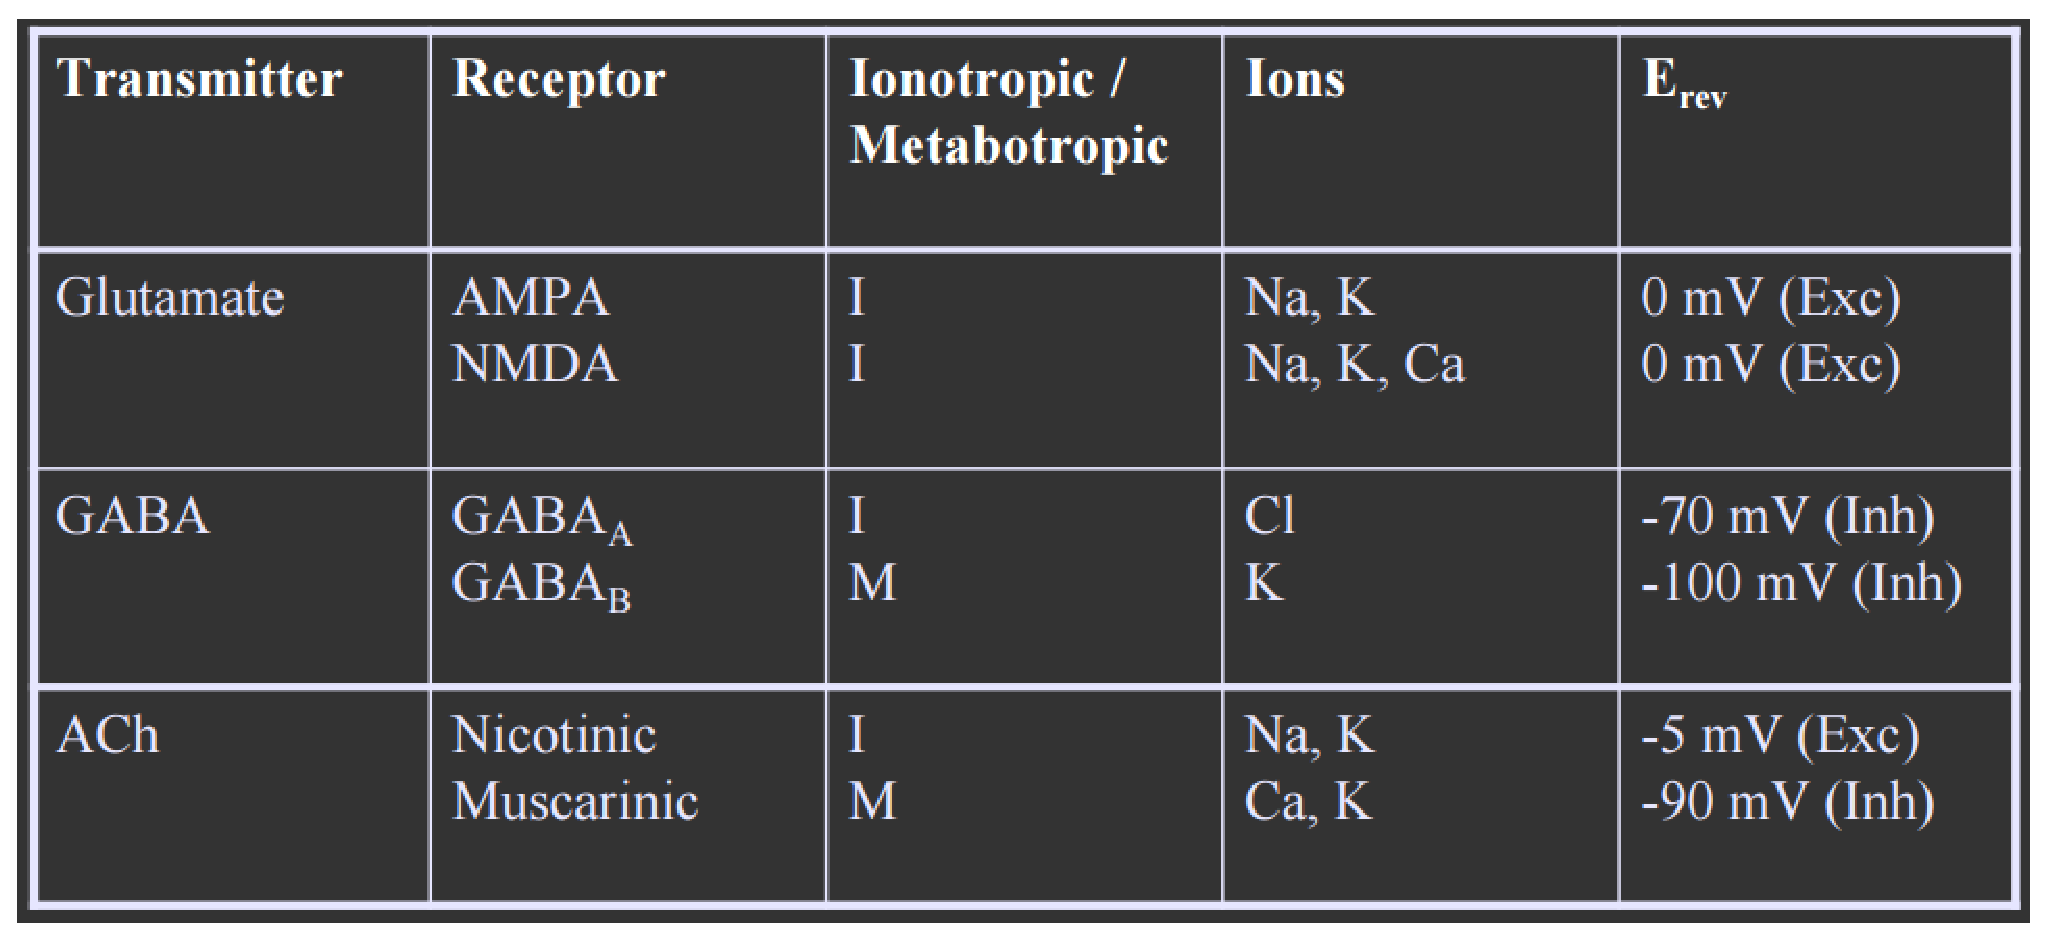
\includegraphics[height=5cm]{./images/synaptic-input.eps}}
    \caption{The different types of (post)synaptic
    input}\label{fig:synaptic-input}
\end{figure}


\textcolor{red}{Deterministic approach}:
So the postsynaptic input current (generated by the
activity of neurotransmitter leading to the opening of receptors such as AMPAR,
NMDAR, mGluR \ldots) can be modelled as
\begin{equation}
I_{\post,i}(t) = g_{\post,i} (V_m - E_{\rev,i}) 
\end{equation}
with $i$ represent one of the above receptors, i.e. a type of synaptic input.

Depending on the type of synaptic input, a functional form is used representing
the activating at a certain time point $t_{\spike, i}$ and decay over time
\begin{equation}
I_{\post,i}(t) = g_{\post,i}(t-t_{\spike,i}) \times (V_m - E_{\rev,i})
\end{equation}

\begin{enumerate}
  \item single exponential

\begin{equation}
g_{\post,i}(t) = \bar{g} \times e^{-t\tau_i}
\end{equation}  

  \item $\alpha$-Function
  
\begin{equation}
g_{\post,i}(t)  = \bar{g} \times t \times e^{-t\tau_{\peak,i}}
\end{equation} 

  \item double exponential ($t_1> t_2$)  
\begin{equation}
g_{\post,i}(t)  = \bar{g} \times \left( e^{-t/\tau_1} - e^{-t/\tau_2} \right)
\end{equation}  
\end{enumerate} 
REMEMBER: $g(t) = 0$ (for $t< 0$)

\section{Algorithms of synaptic modification}
%\label{sec:synaptic_strength}


\subsection{LTP}

LTP has been most widely studied in hippocampus, with glutamate
neurotransmitters involved in Schaffer collateral/CA1 pyramidal cell pathway.

\textcolor{red}{The goal of understanding different algorithms of synaptic
modification is to understand synaptic efficacy, functional coupling, adaptive
change in behavior.}
\begin{itemize}
  \item metabolic changes
\begin{enumerate}
  \item changes from presynaptic side
  
  \begin{itemize}
    \item  more neurontransmitter vesicles
  release)? 
  
  increase glutamate release found in axonal branches (Schaffer collaterals)
  projecting to CA1 pyramids {\it in vitro} \citep{skrede1981}, and in perforant
  path {\it in vivo} \citep{dolphin1982}.
     
     \item 
  \end{itemize}
  
  \item changes from postsynaptic side 
  
  \begin{itemize}
    \item NMDAR and/or AMPAR more sensitive to
  neurotransmitter binding
  
  in which LTP is accompanied by a prolonged increase in $\Ca$ uptake
  
     \item increase in the number of postsynaptic receptors
     
     during the ``firing", some how more 
     glutamate receptors (Sect.\ref{sec:glutamate_receptor}) are available
     \citep{baudry1980}
      
     AMPAR are inserted which makes the
     depolarization stronger;  and these AMPR are not removed unless some thing
     happens
     
     \item any metabolic changes inside postsynaptic that makes the depolarization easier
     
     \item \ldots
  \end{itemize}
  
  \item both ?
\end{enumerate}

  \item retrograde signalling: from postsynaptic side the induced change in
  neurotransmitter release on presynaptic side?
  
  \item growth factor ?
  \begin{enumerate}
    \item spines head growth in volume
    \item spine neck growth in volume
    \item spines split into two connections.
  \end{enumerate}
\end{itemize}

\subsection{LTD}



\textcolor{red}{The goal of understanding different algorithms of synaptic
modification is to understand synaptic efficacy, functional coupling, adaptive
change in behavior.}
\begin{itemize}
  \item metabolic changes
\begin{enumerate}
  \item changes from presynaptic side
  
  \begin{itemize}
    \item  more neurontransmitter vesicles
  release)? 
  
     \item 
  \end{itemize}
  
  \item changes from postsynaptic side 
  
  \begin{itemize}
    \item NMDAR and/or AMPAR less sensitive to  neurotransmitter binding
  
  
     \item reduced in the number of postsynaptic receptors
     
     \item any metabolic changes inside postsynaptic that makes the depolarization easier
     
     \item \ldots
  \end{itemize}
  
  \item both ?
\end{enumerate}

  \item retrograde signalling: postsynaptic side induces the inhibition
  of neurotransmitter release on presynaptic side?
  
  \item growth factor ?
  \begin{enumerate}
    \item spines head growth in volume
    \item spine neck growth in volume
    \item spines split into two connections.
  \end{enumerate}
\end{itemize}

\textcolor{red}{It reduces the number of AMPA receptors at the synapse}. HOW???

LTD is induced by a minimum level of postsynaptic depolarization (i.e. weak
stimulation). Induction of LTD can be 
\begin{itemize}
  \item {\bf NMDAR suppression induced LTD}: NMDAR-dependent in the hippocampal
CA1 region and, like LTP induction, requires $\Ca$ influx through NMDARs
\citep{bear1994} of synaptic transmission (Sect.\ref{sec:synaptic_transmission})
in many areas of the brain.

The mechanism by which NMDAR-dependent LTD reduces synaptic strength is to
reverse the effects of LTP: dephosphorylation of AMPARs, thus reducing their
open probability and removal of AMPARs from the synaptic plasma membrane by
endocytosis.

   \item {\bf mGluR-dependent LTD}: LTD is induced by stimulation of
   metabotropic glutamate receptors (Sect.\ref{sec:mGluR})
   \citep{bortolotto1999}.

  \item  {\bf endocannabinoid-mediated LTD} \citep{Sjostrom2003}
  
\end{itemize}

$V_m$-dependent $\Ca$ channels (VDCC) is important to LTD, i.e. inhibition of
VDCC tends to suppress LTD.

There are also two phases in LTD. Like late phase in LTP, late phase in LTD also
require protein synthesis. However, \textcolor{red}{much less is known about
late phase in LTD.}

\subsection{ * I-V equation at single synapse}
\label{sec:synapse_I-V-curve}

So, the I-V equation on postsynaptic side is
\begin{equation}
\Csc \frac{dV_m}{dt} = -g_\na(V_m-E_\na) - g_\K (V_m - E_\K) - g_\Cl (V_m -
V_\Cl) - \sum g_{\post, i} (V_m - E_{\rev,i}) + I_\app
\end{equation}
with $I_\app$ is the applied current or injected current in the experiment to 
represent the membrane change due to the binding of neurotransmitter
released from presynaptic side.






